\chapter{Question 1}
\label{intro}

\textbf{We know the result of the Karate Club (Zachary, 1977) split. Prove or disprove that the result of split could have been predicted by the weighted graph of social interactions.  How well does the mathematical model represent reality?
Generously document your answer with all supporting equations, code, graphs, arguments, etc.
Useful sources include:}

\textbf{* Original paper}\\
\url{http://aris.ss.uci.edu/~lin/76.pdf}\\
\textbf{* Slides}\\
\url{http://www-personal.umich.edu/~ladamic/courses/networks/si614w06/ppt/lecture18.ppt}\\
\url{http://clair.si.umich.edu/si767/papers/Week03/Community/CommunityDetection.pptx}\\
\textbf{* Code and data}\\
\url{http://networkx.github.io/documentation/latest/examples/graph/karate_club.html}\\
\url{http://nbviewer.ipython.org/url/courses.cit.cornell.edu/info6010/resources/11notes.ipynb}\\
\url{http://stackoverflow.com/questions/9471906/what-are-the-differences-between-community-detection-algorithms-in-igraph/9478989#9478989}\\
\url{http://stackoverflow.com/questions/5822265/are-there-implementations-of-algorithms-for-community-detection-in-graphs}\\
\url{http://konect.uni-koblenz.de/networks/ucidata-zachary}\\
\url{http://vlado.fmf.uni-lj.si/pub/networks/data/ucinet/ucidata.htm#zachary}\\
\url{https://snap.stanford.edu/snappy/doc/reference/CommunityGirvanNewman.html}\\
\url{http://igraph.org/python/doc/igraph-pysrc.html#Graph.community_edge_betweenness}

\newpage
Following are the steps I have taken to solve the given problem:
\begin{itemize}
\item To understand about the Karate Club split (Zachary, 1977) I read the original paper from \url{http://aris.ss.uci.edu/~lin/76.pdf} which explains the reason behind the split and also illustrates the graphical and matrix representation of the social relationships among the 34 individuals in the karate club.
\item Looking at week 6 PowerPoint slides `Social Networks' I understood the difference between strong and weak ties, results of removing strong and weak ties and also some general approaches like `Divisive method' and `Agglomerative method' for partitioning a graph.
\item After researching all the sources provided, I decided to solve this problem using the Divisive method proposed by `Girvan' and `Newman' which uses the concept of `edge betweenness' to identify which edge to be removed.
\item I downloaded the data for Karate Club in GraphML format.
\item To implement the Girvan Newman algorithm and produce the graphs I installed an open source library `python-igraph' which is a network analysis tool that has large set of graph generators, layout methods to visualize a graph, and also built-in routines to calculate centrality properties like edge and vertex betweenness. 
\newpage
\item I wrote a Python code that reads the GraphML file and plots the Original Graph without any split which is illustrated in Figure \ref{fig:q1fig00} and a graph which distinguishes the Karate Club split based on faction which is in Figure \ref{fig:q1fig01}.
\begin{figure}[h!]
\begin{center}
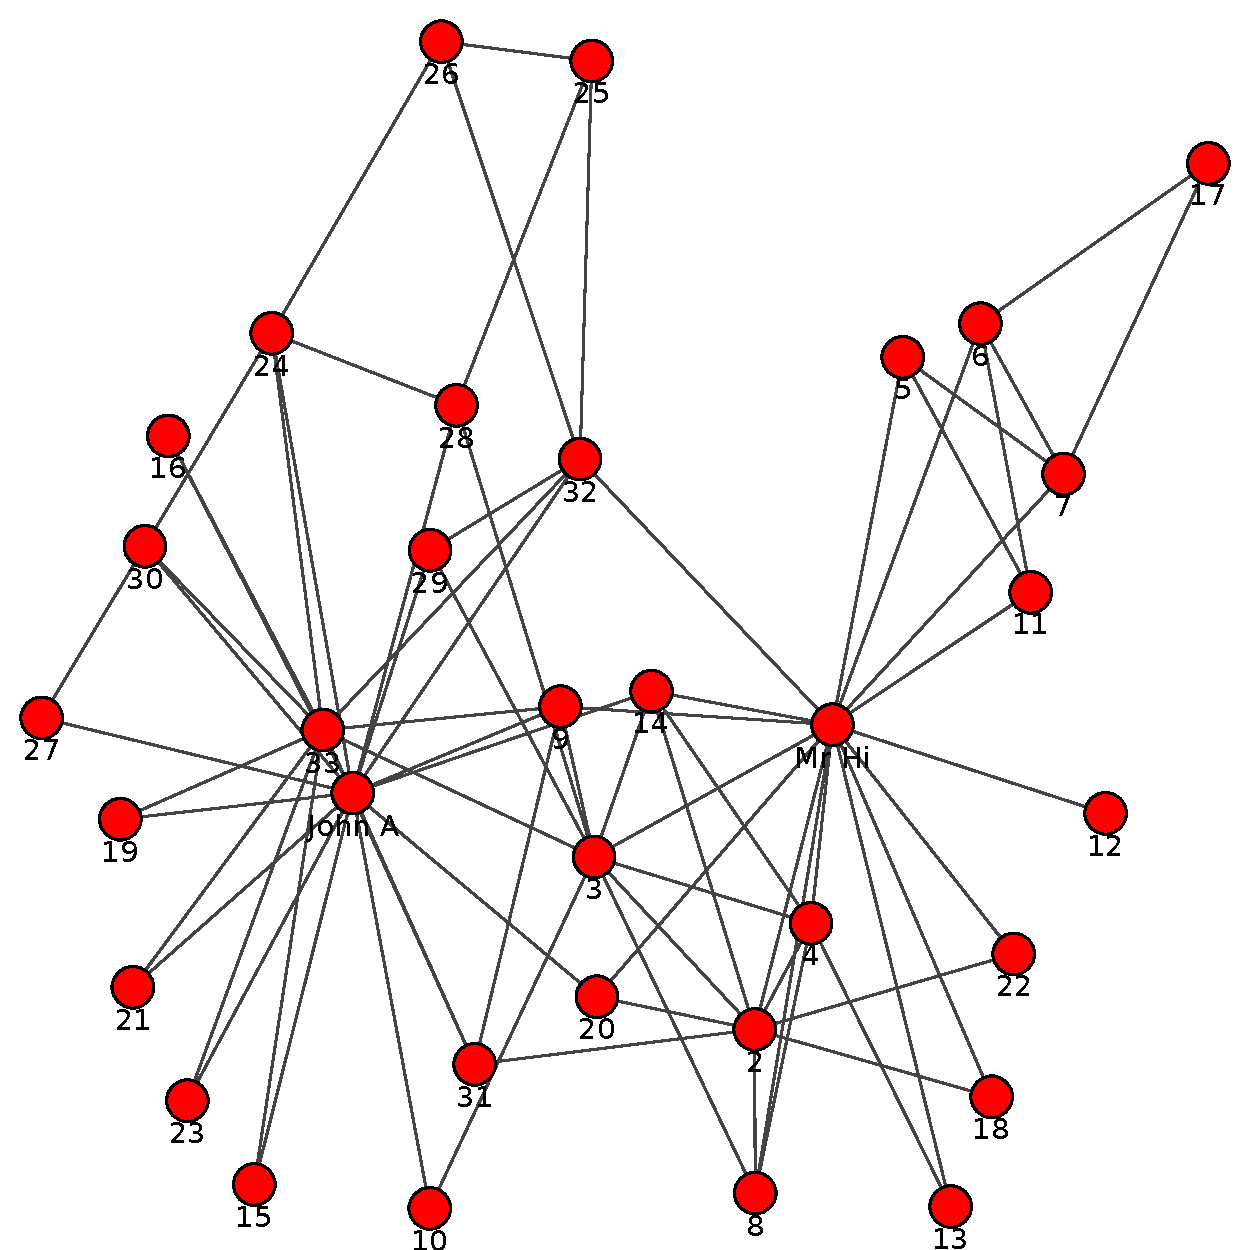
\includegraphics[scale=0.55, keepaspectratio=true]{figures/graphs/OriginalGraph.pdf}
\caption{Original Graph without any split}
\label{fig:q1fig00}
\end{center}
\end{figure}
\newpage
\begin{figure}[h!]
\begin{center}
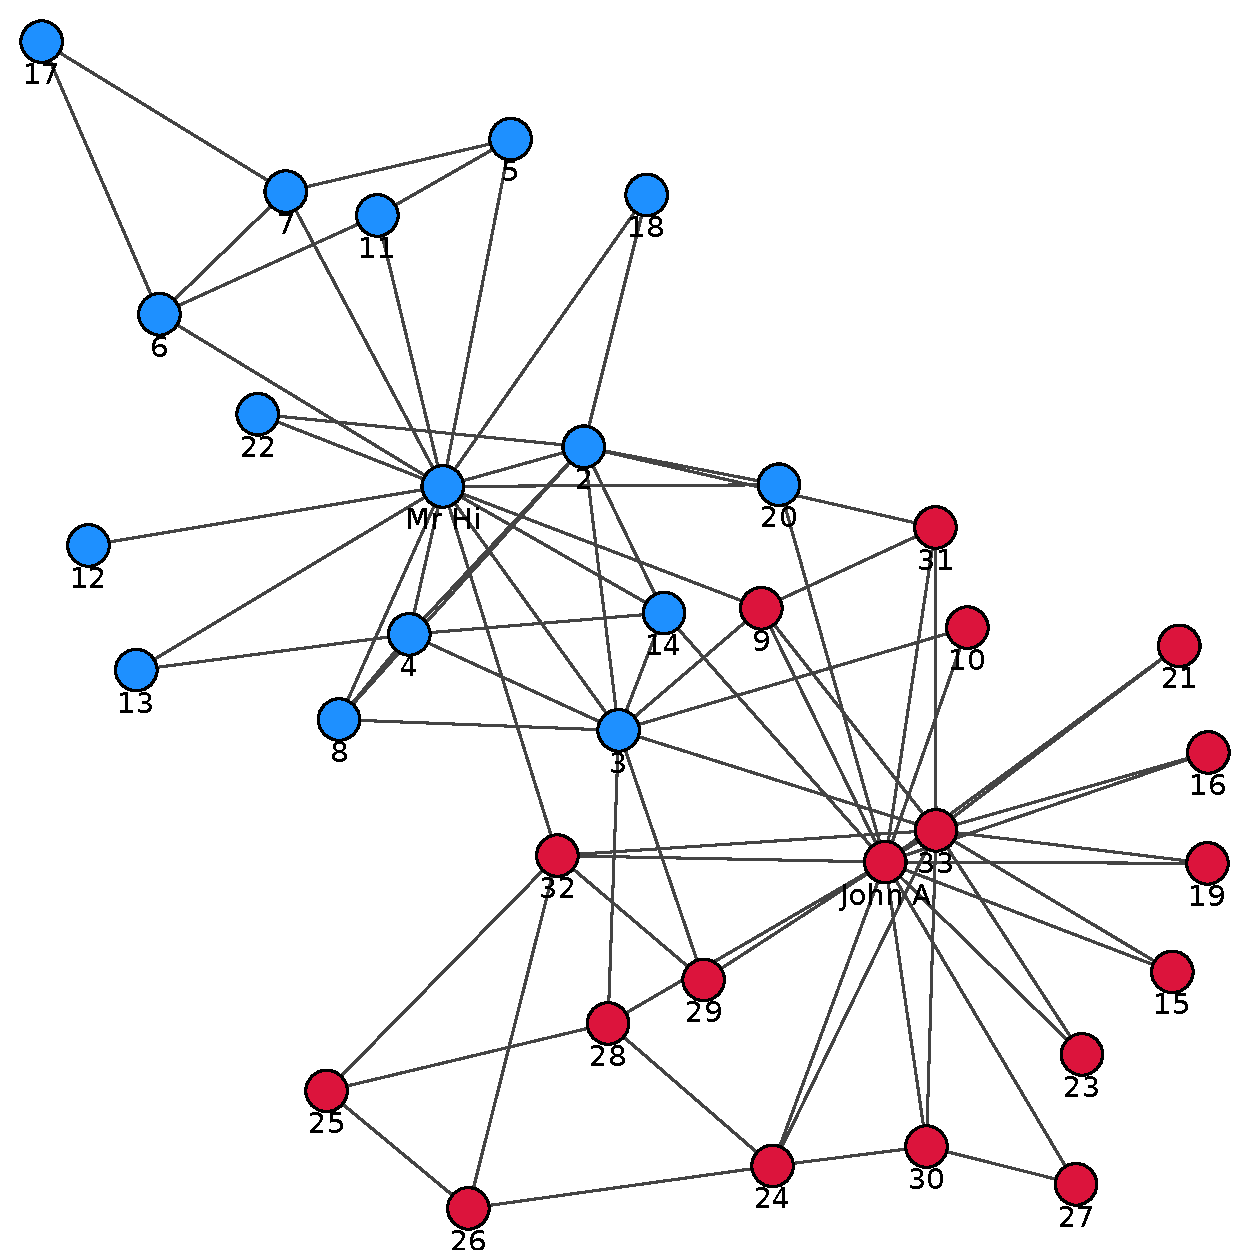
\includegraphics[scale=0.55, keepaspectratio=true]{figures/graphs/FactionGraph.pdf}
\caption{Graph which distinguishes two groups based on Faction}
\label{fig:q1fig01}
\end{center}
\end{figure}
\item Furthermore, I calculated the edge betweenness for all the edges in the graph
\newpage
\item In each iteration the edges with highest betweenness is highlighted in `red' and then deleted until graph is partitioned into as many regions as desired. These graphs are illustrated in Figures \ref{fig:q1fig1}, \ref{fig:q1fig2}, \ref{fig:q1fig3}, \ref{fig:q1fig4}, \ref{fig:q1fig5}, \ref{fig:q1fig6}, \ref{fig:q1fig7}, \ref{fig:q1fig8}, \ref{fig:q1fig9}, \ref{fig:q1fig10}, \ref{fig:q1fig11}.
\begin{figure}[h!]
\begin{center}
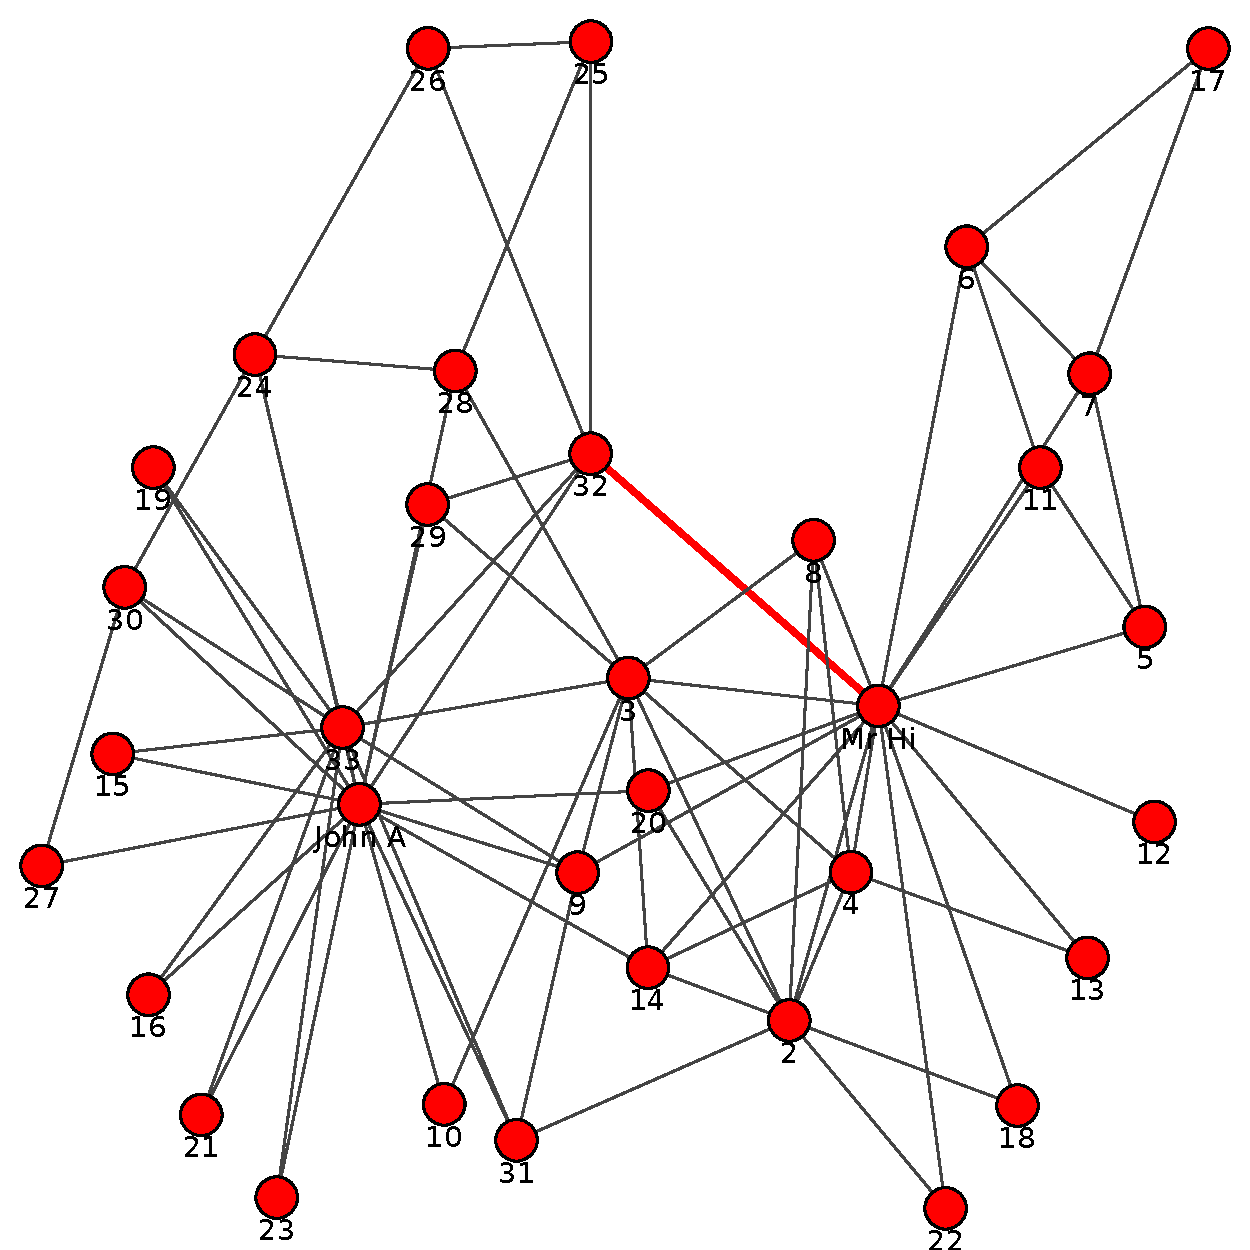
\includegraphics[scale=0.55, keepaspectratio=true]{figures/graphs/EdgeHighlightedGraph1.pdf}
\caption{Iteration 1}
\label{fig:q1fig1}
\end{center}
\end{figure}
\newpage
\begin{figure}[h!]
\begin{center}
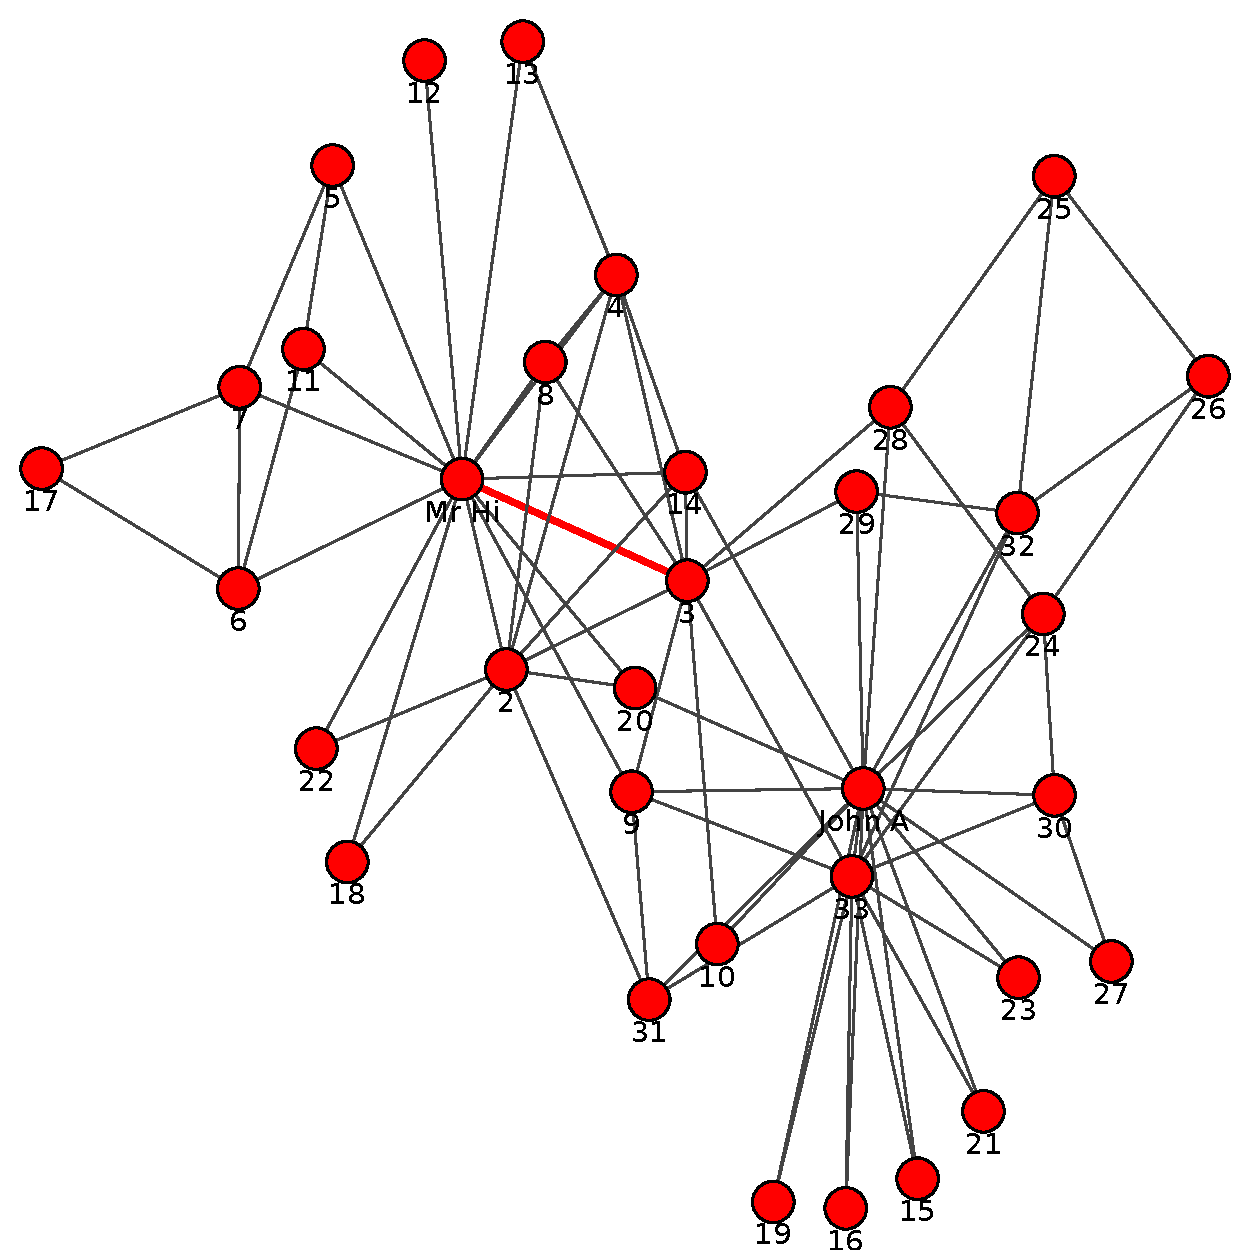
\includegraphics[scale=0.55, keepaspectratio=true]{figures/graphs/EdgeHighlightedGraph2.pdf}
\caption{Iteration 2}
\label{fig:q1fig2}
\end{center}
\end{figure}
\newpage
\begin{figure}[h!]
\begin{center}
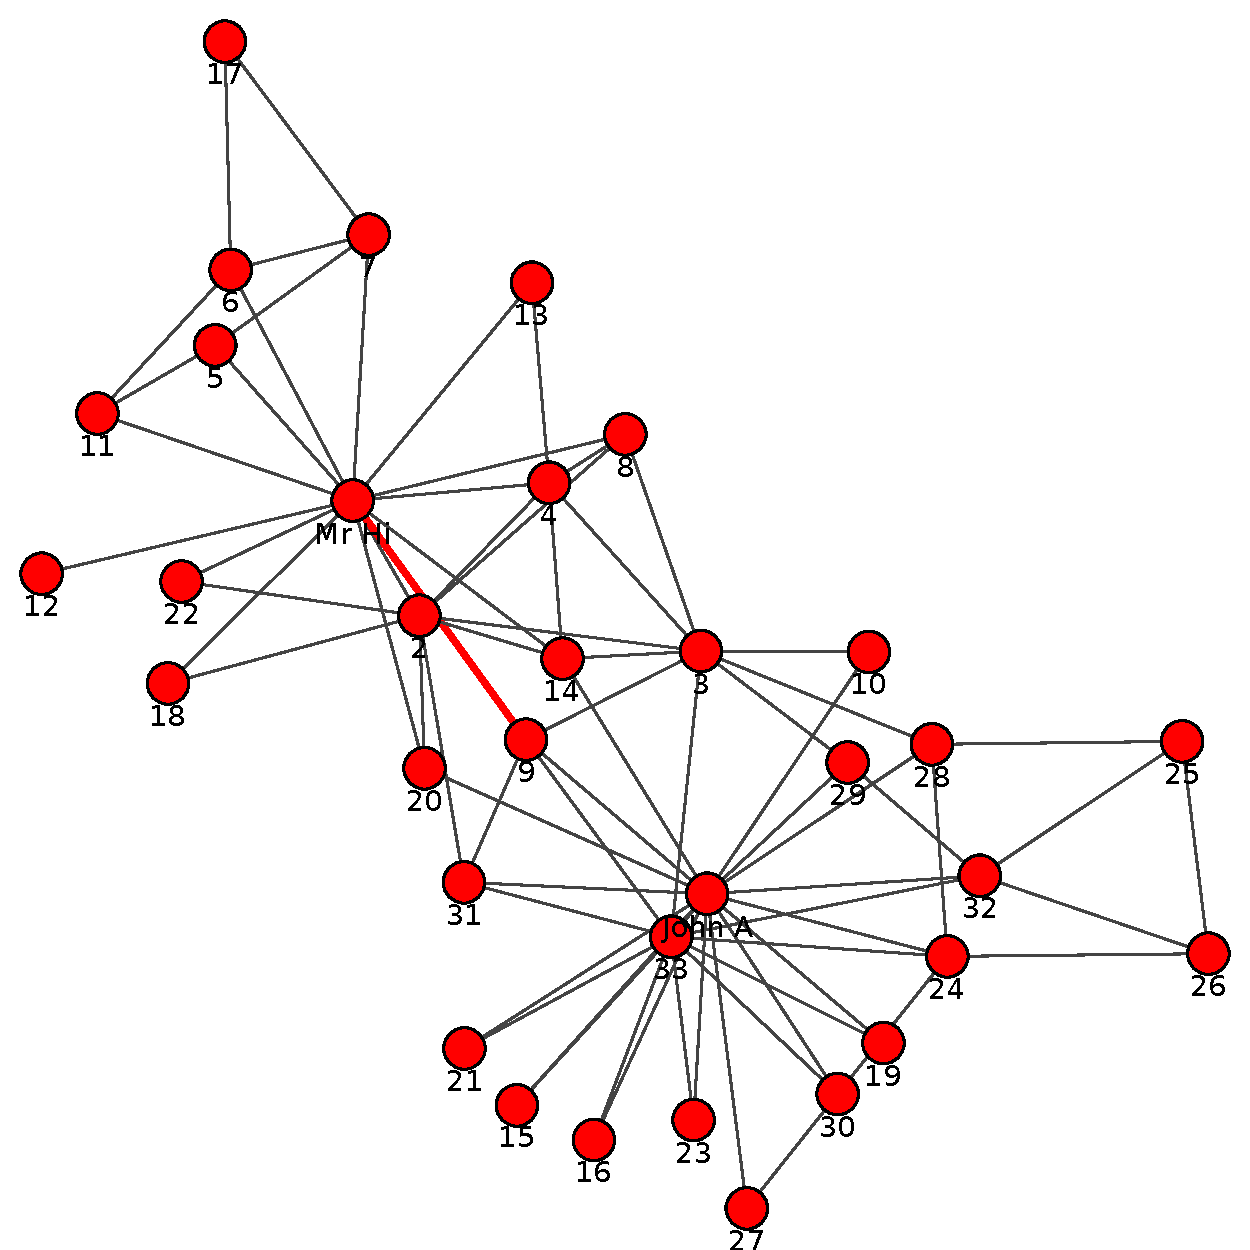
\includegraphics[scale=0.55, keepaspectratio=true]{figures/graphs/EdgeHighlightedGraph3.pdf}
\caption{Iteration 3}
\label{fig:q1fig3}
\end{center}
\end{figure}
\newpage
\begin{figure}[h!]
\begin{center}
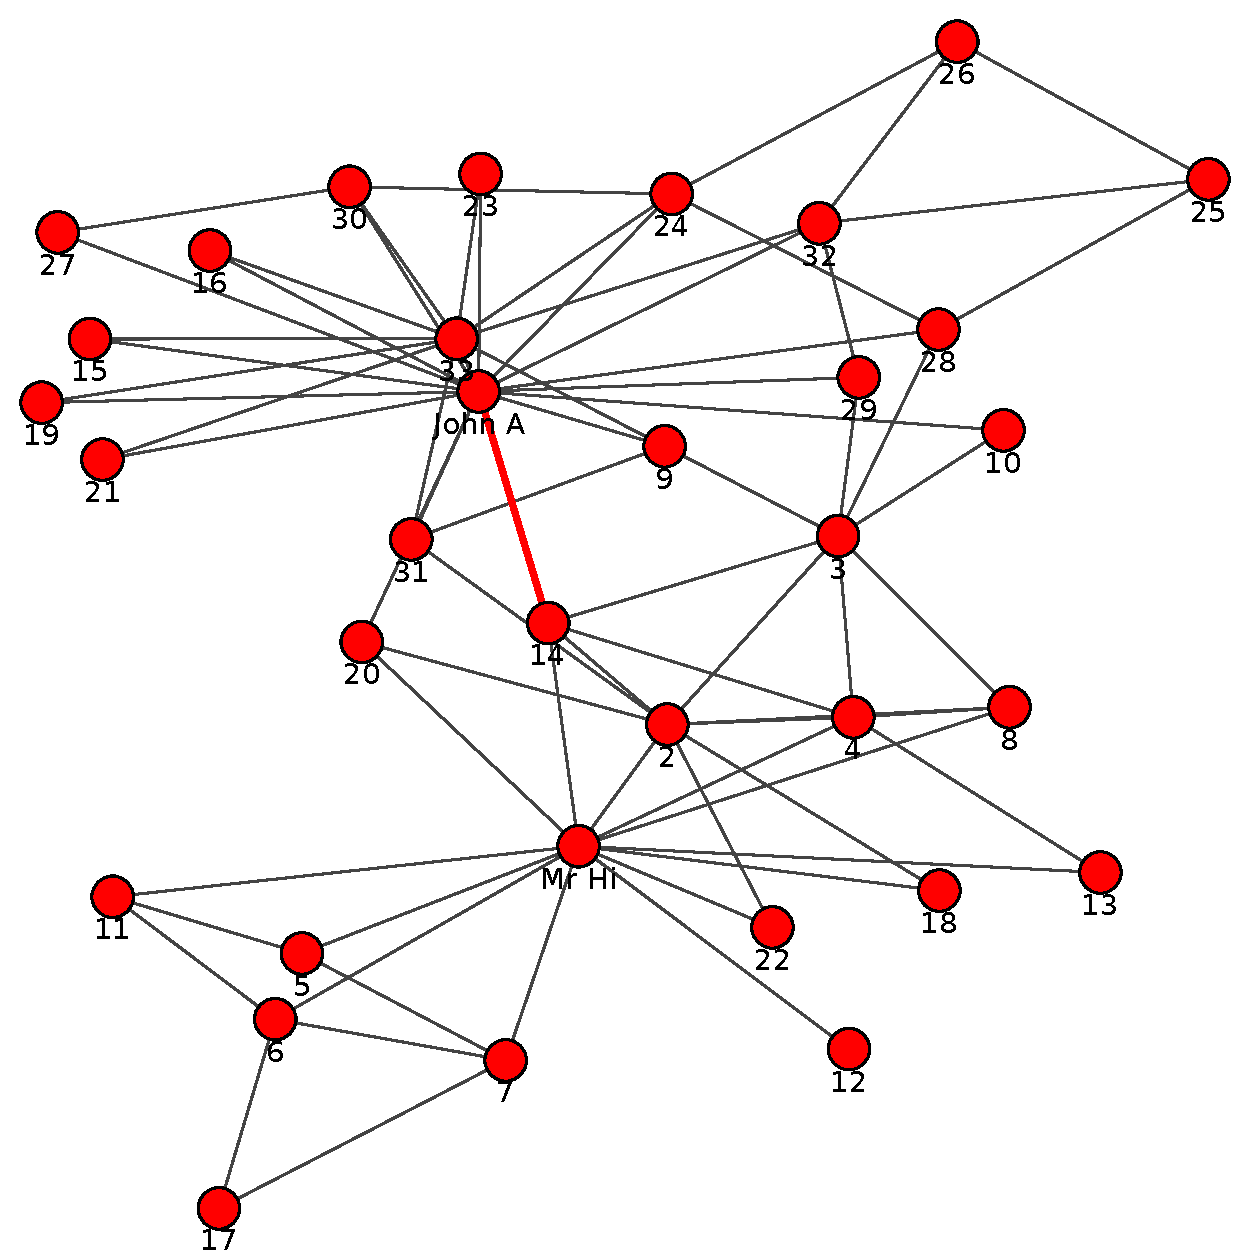
\includegraphics[scale=0.55, keepaspectratio=true]{figures/graphs/EdgeHighlightedGraph4.pdf}
\caption{Iteration 4}
\label{fig:q1fig4}
\end{center}
\end{figure}
\newpage
\begin{figure}[h!]
\begin{center}
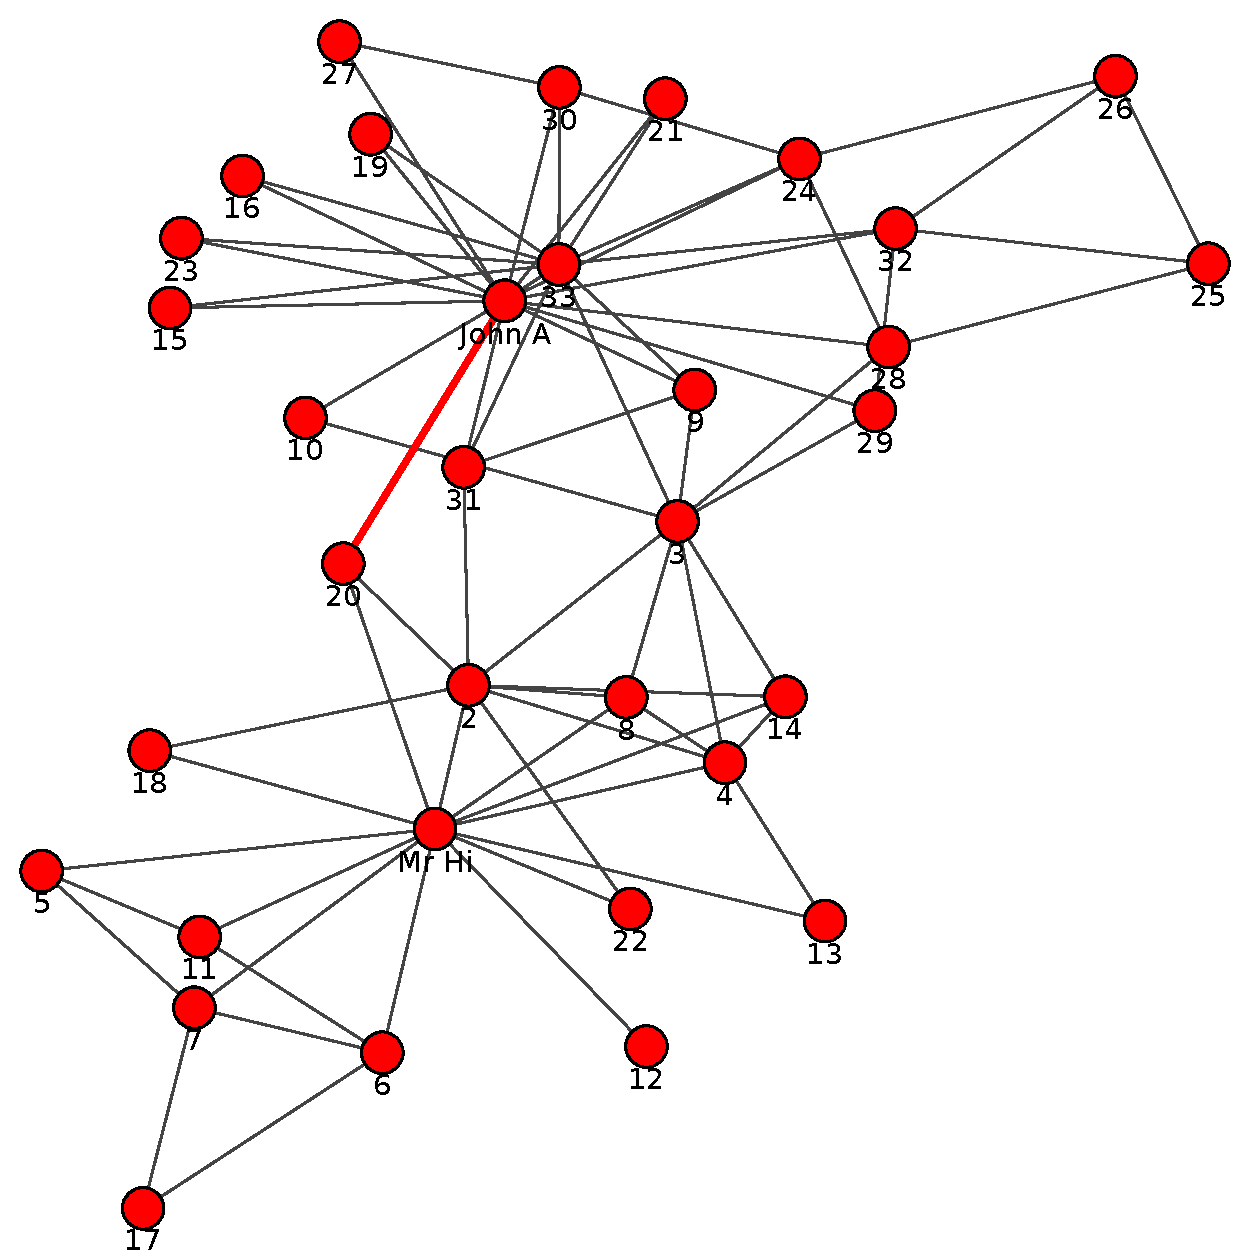
\includegraphics[scale=0.55, keepaspectratio=true]{figures/graphs/EdgeHighlightedGraph5.pdf}
\caption{Iteration 5}
\label{fig:q1fig5}
\end{center}
\end{figure}
\newpage
\begin{figure}[h!]
\begin{center}
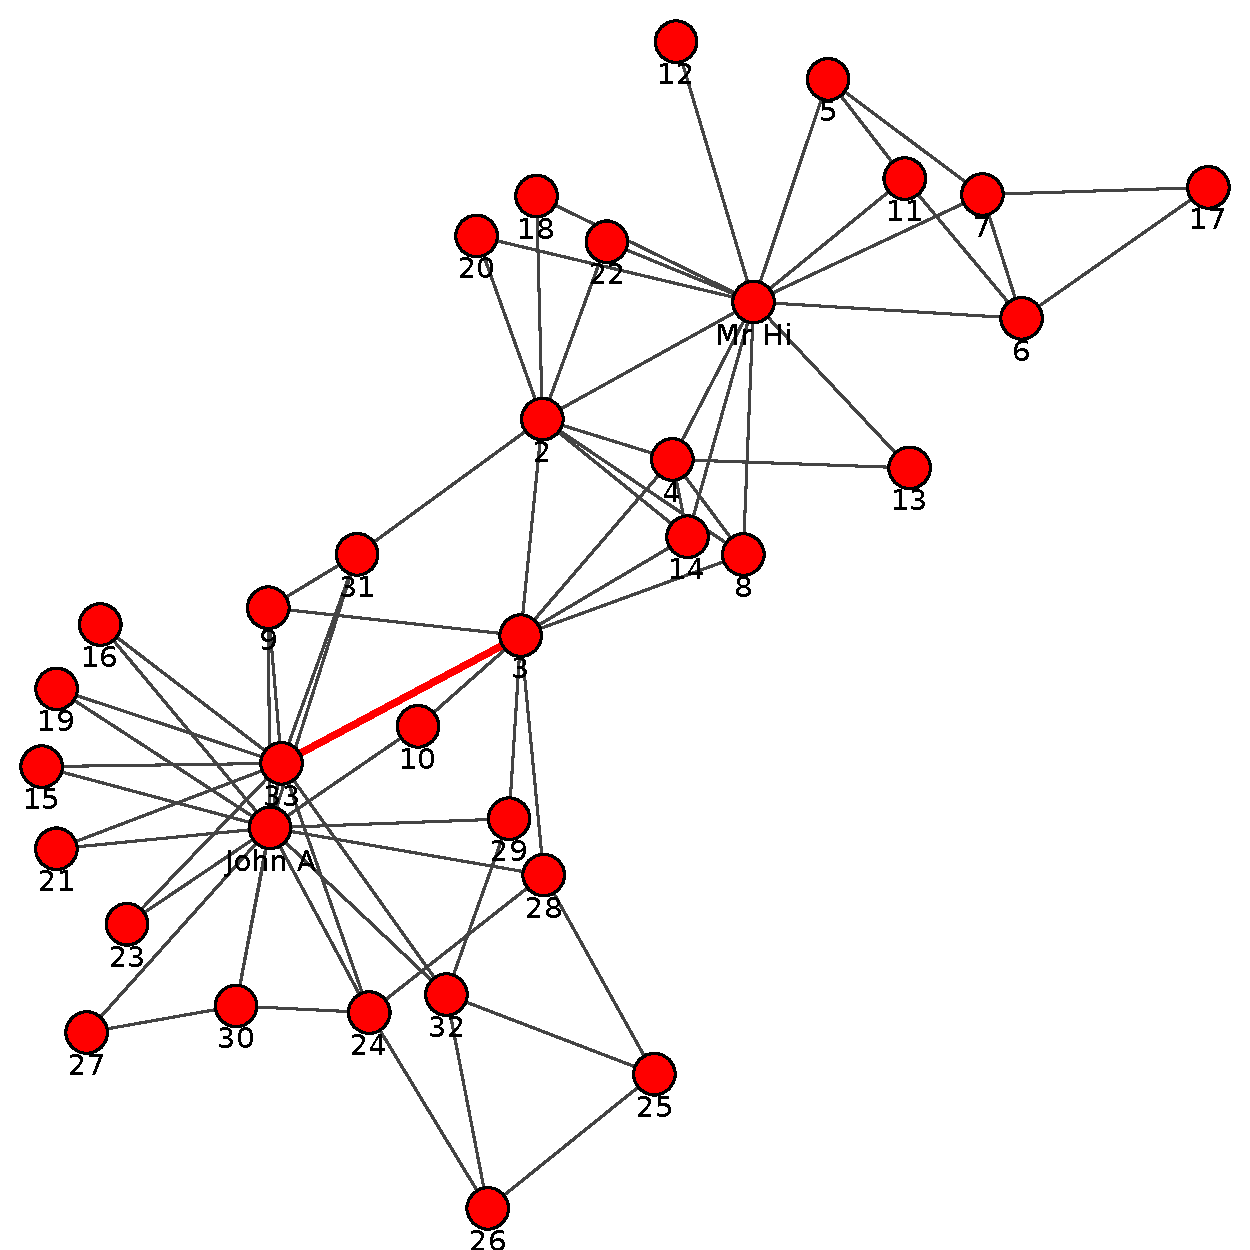
\includegraphics[scale=0.55, keepaspectratio=true]{figures/graphs/EdgeHighlightedGraph6.pdf}
\caption{Iteration 6}
\label{fig:q1fig6}
\end{center}
\end{figure}
\newpage
\begin{figure}[h!]
\begin{center}
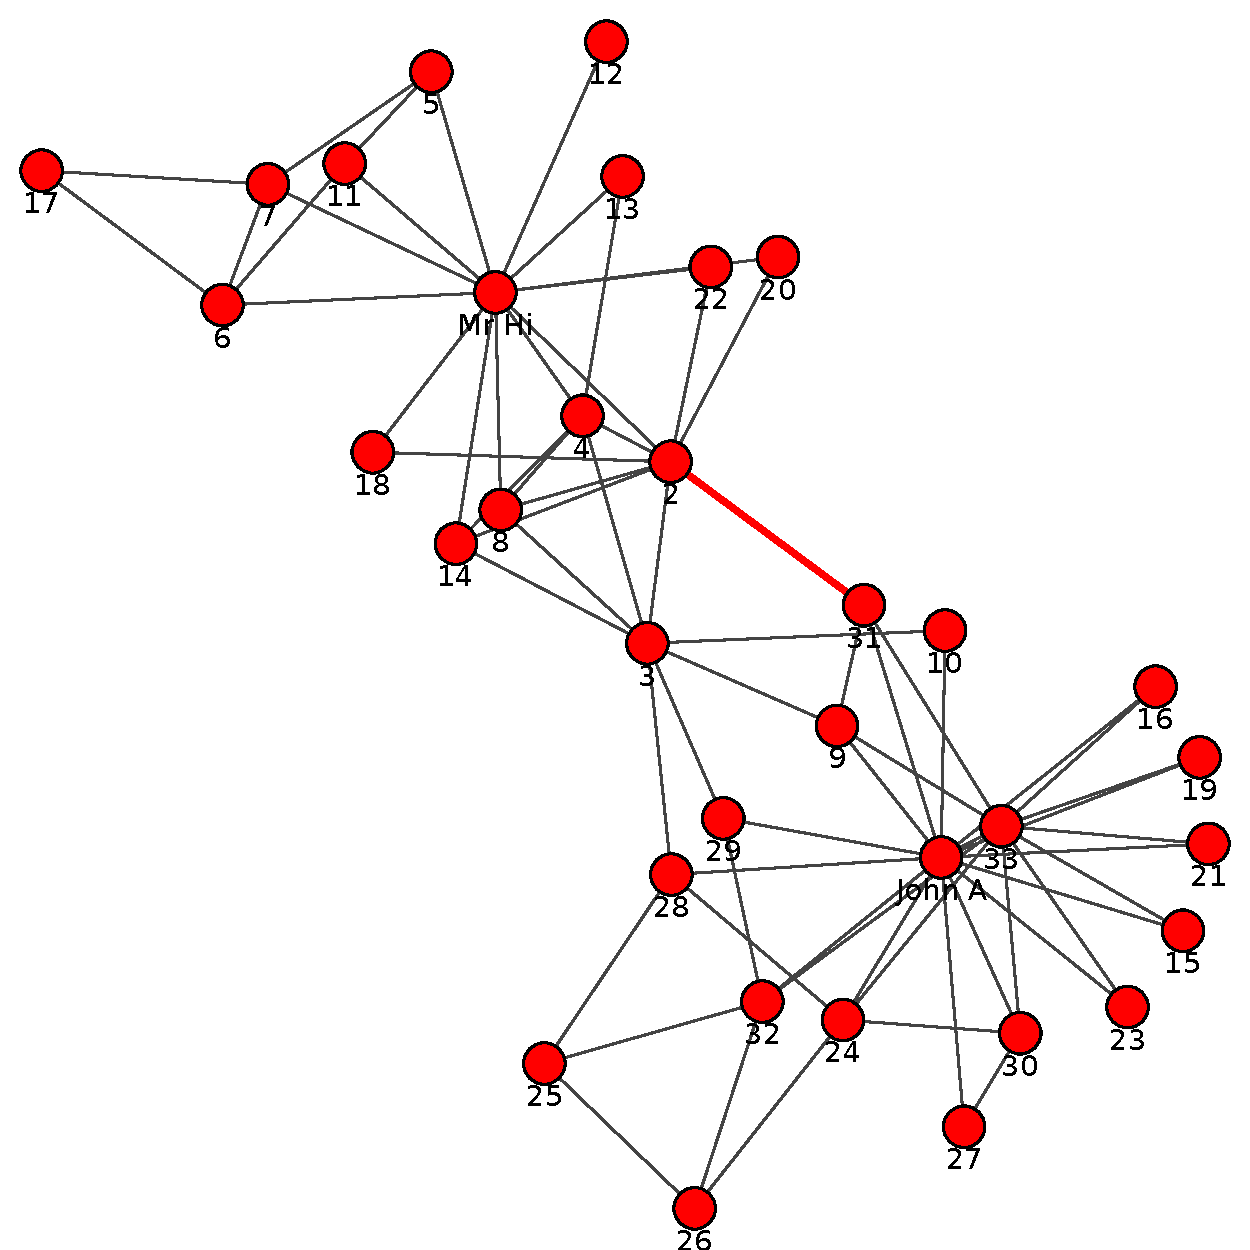
\includegraphics[scale=0.55, keepaspectratio=true]{figures/graphs/EdgeHighlightedGraph7.pdf}
\caption{Iteration 7}
\label{fig:q1fig7}
\end{center}
\end{figure}
\newpage
\begin{figure}[h!]
\begin{center}
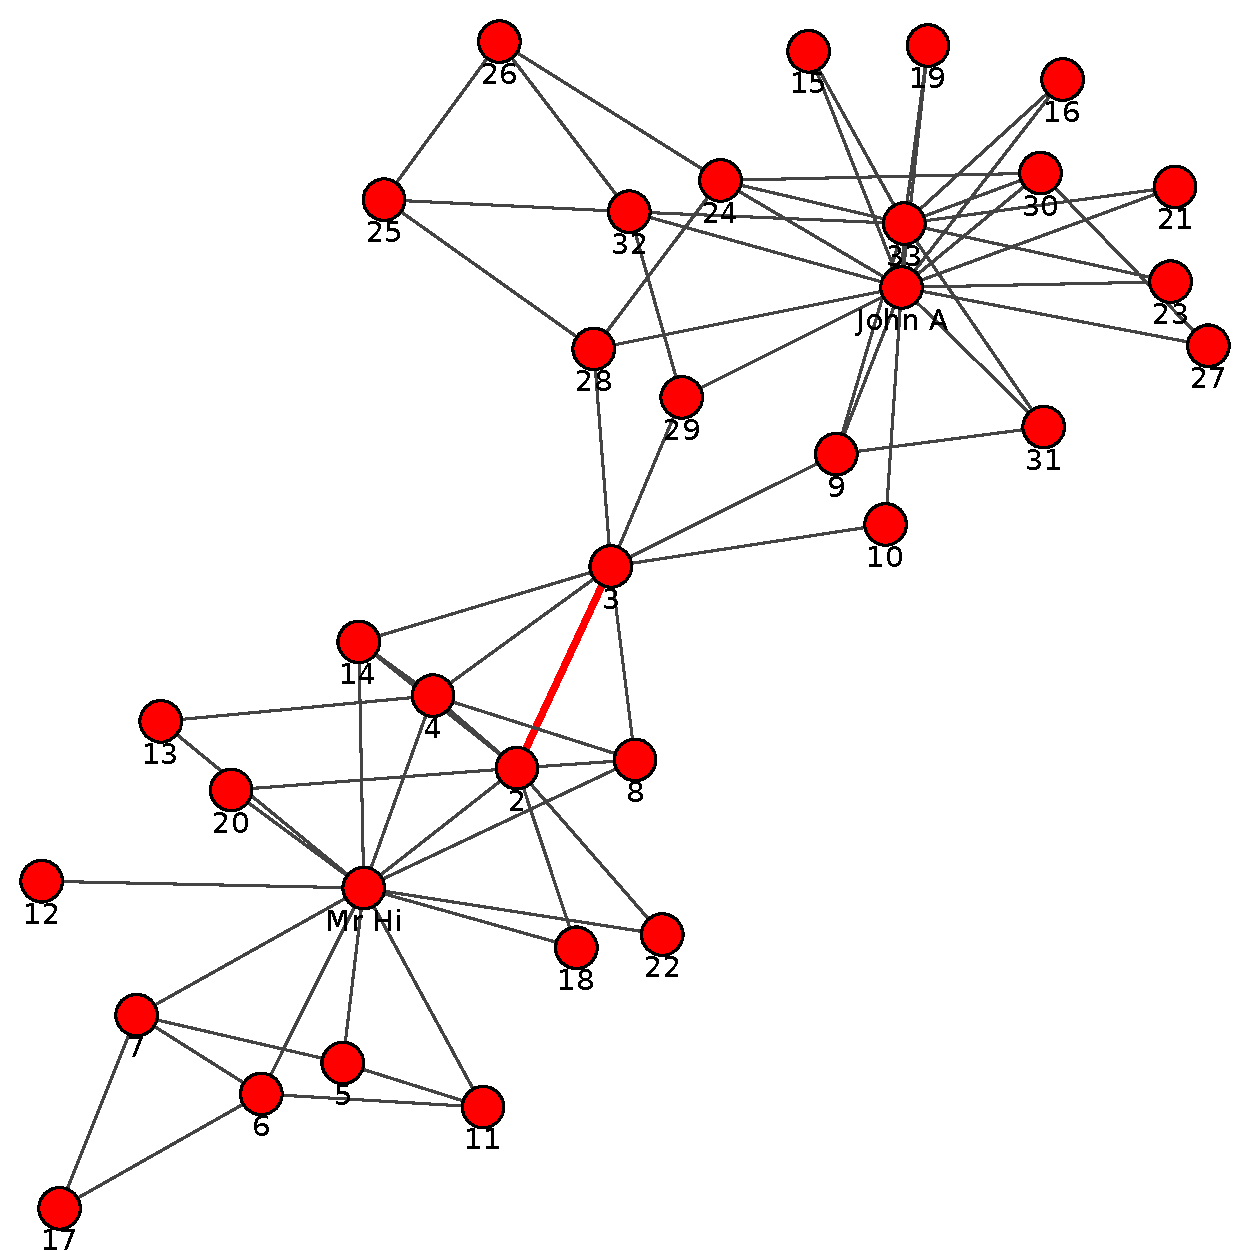
\includegraphics[scale=0.55, keepaspectratio=true]{figures/graphs/EdgeHighlightedGraph8.pdf}
\caption{Iteration 8}
\label{fig:q1fig8}
\end{center}
\end{figure}
\newpage
\begin{figure}[h!]
\begin{center}
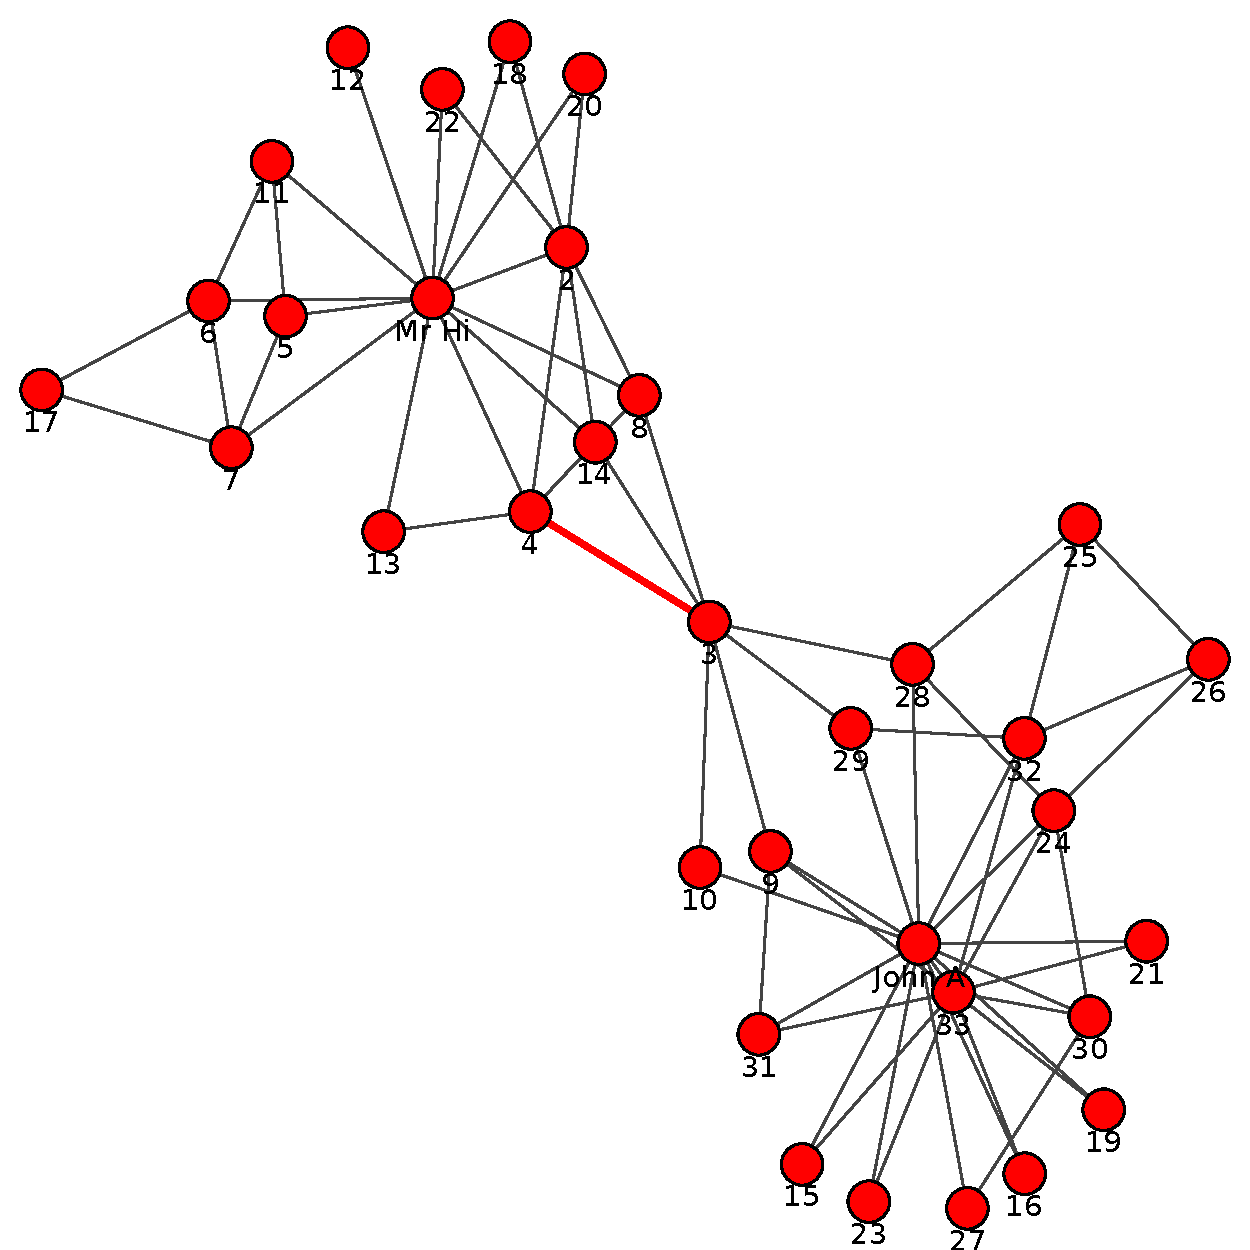
\includegraphics[scale=0.55, keepaspectratio=true]{figures/graphs/EdgeHighlightedGraph9.pdf}
\caption{Iteration 9}
\label{fig:q1fig9}
\end{center}
\end{figure}
\newpage
\begin{figure}[h!]
\begin{center}
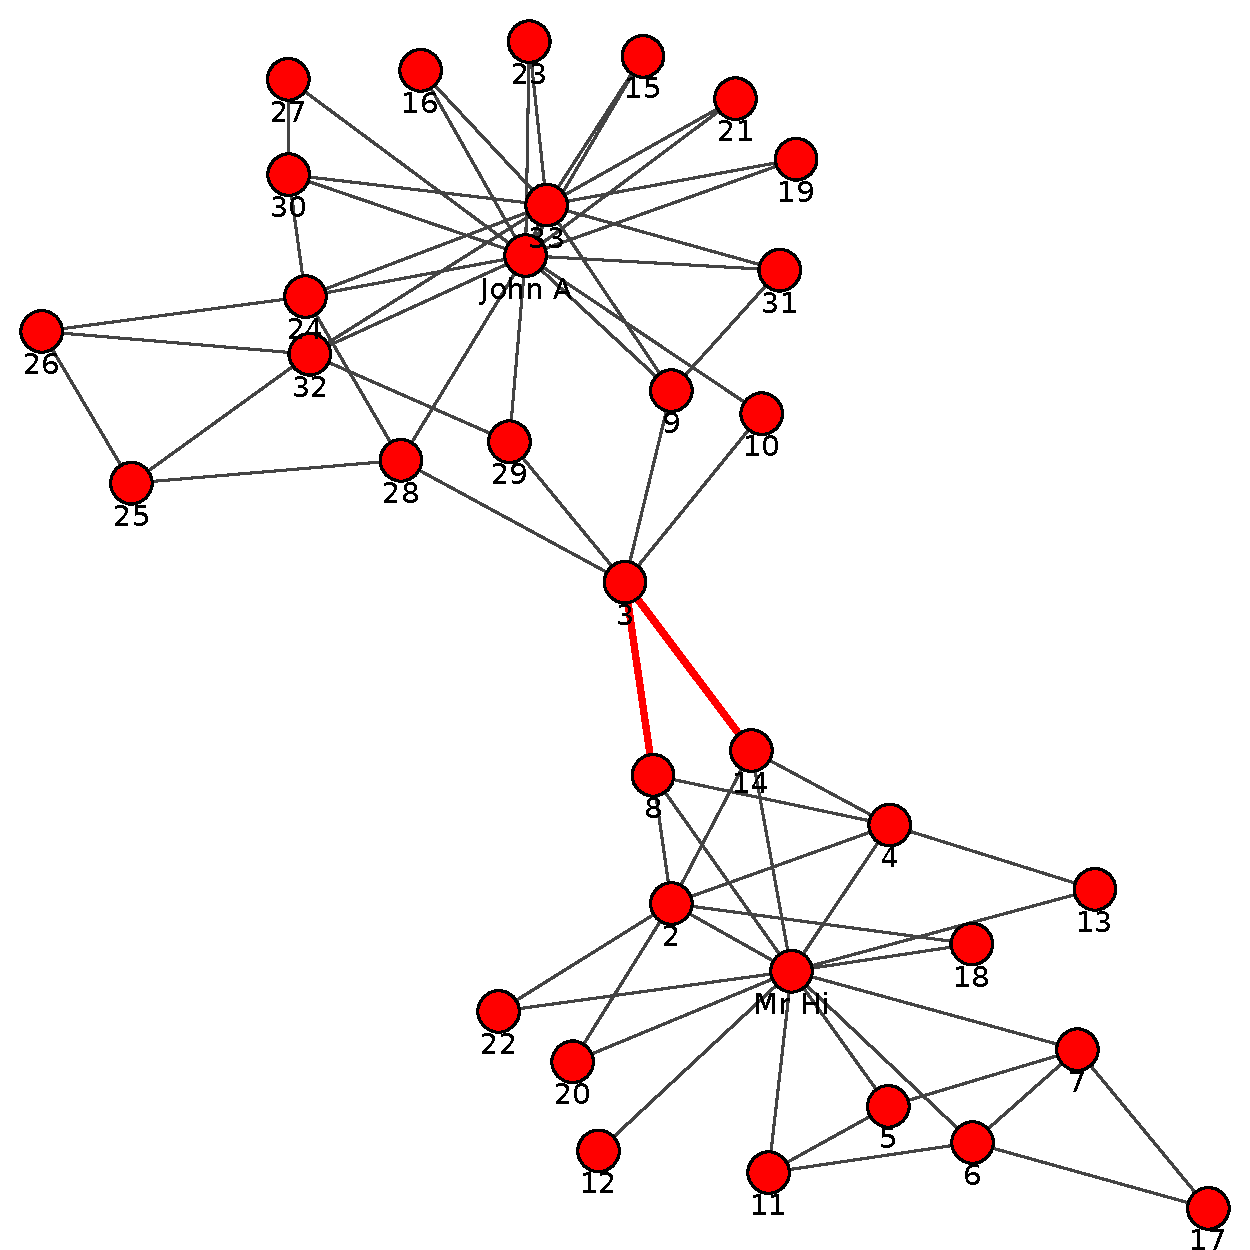
\includegraphics[scale=0.55, keepaspectratio=true]{figures/graphs/EdgeHighlightedGraph10.pdf}
\caption{Iteration 10}
\label{fig:q1fig10}
\end{center}
\end{figure}
\newpage
\begin{figure}[h!]
\begin{center}
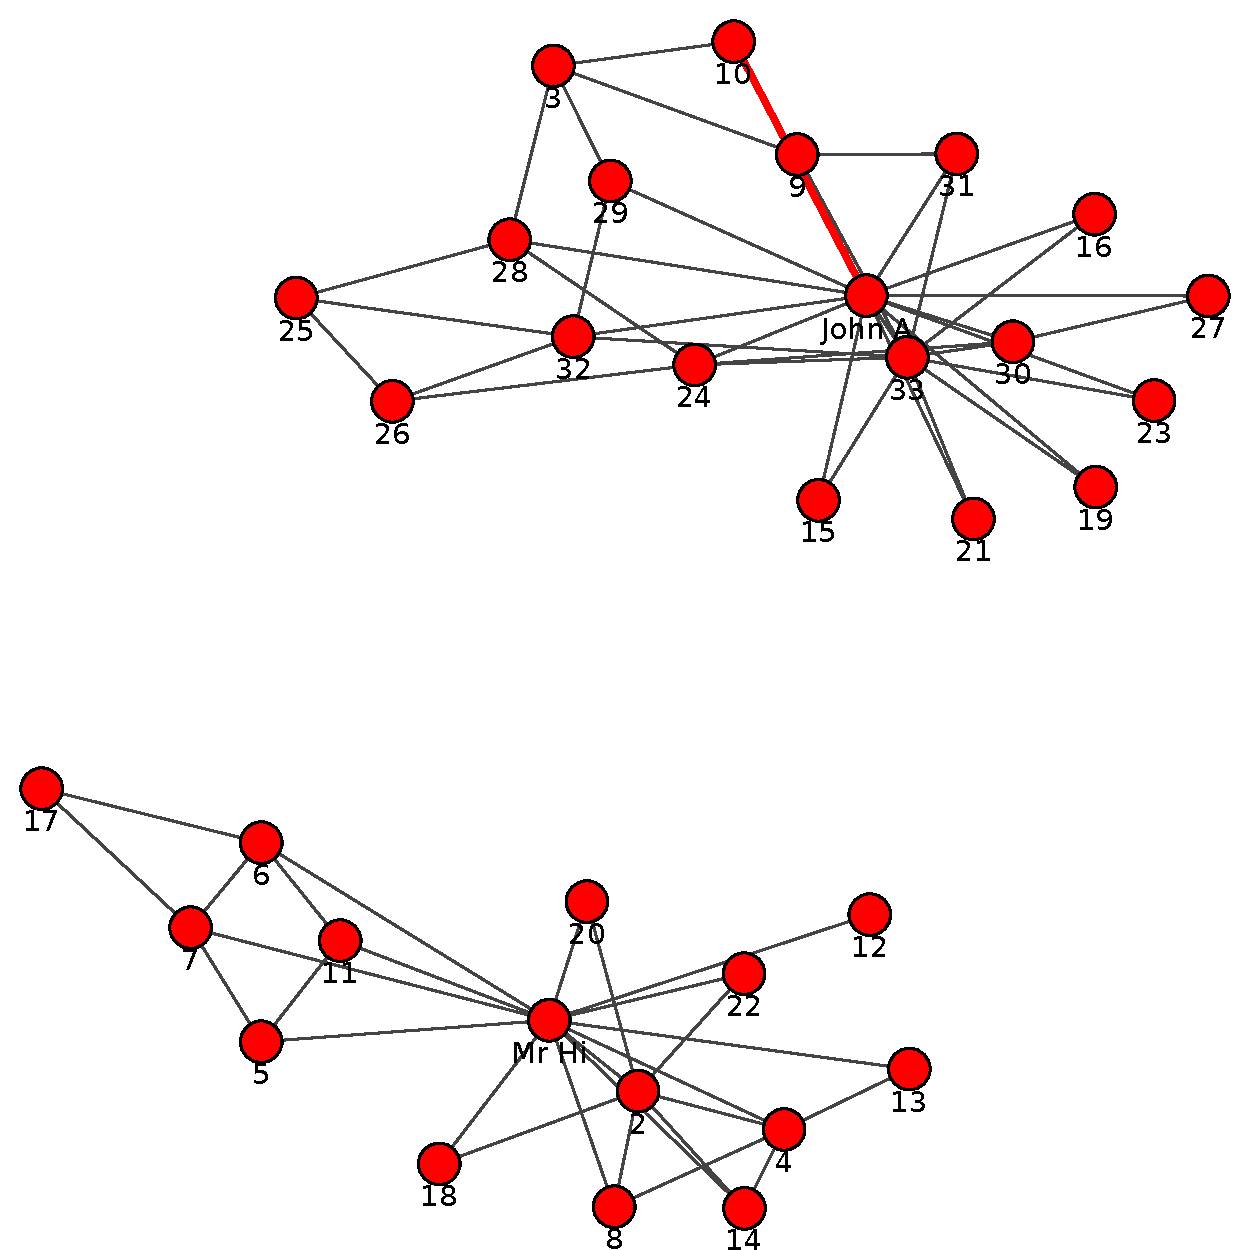
\includegraphics[scale=0.55, keepaspectratio=true]{figures/graphs/EdgeHighlightedGraph11.pdf}
\caption{Iteration 11}
\label{fig:q1fig11}
\end{center}
\end{figure}
\newpage
\item After 11 iterations, the graph is partitioned into 2 groups which is illustrated in Figure \ref{fig:q1fig12}.
\begin{figure}[h!]
\begin{center}
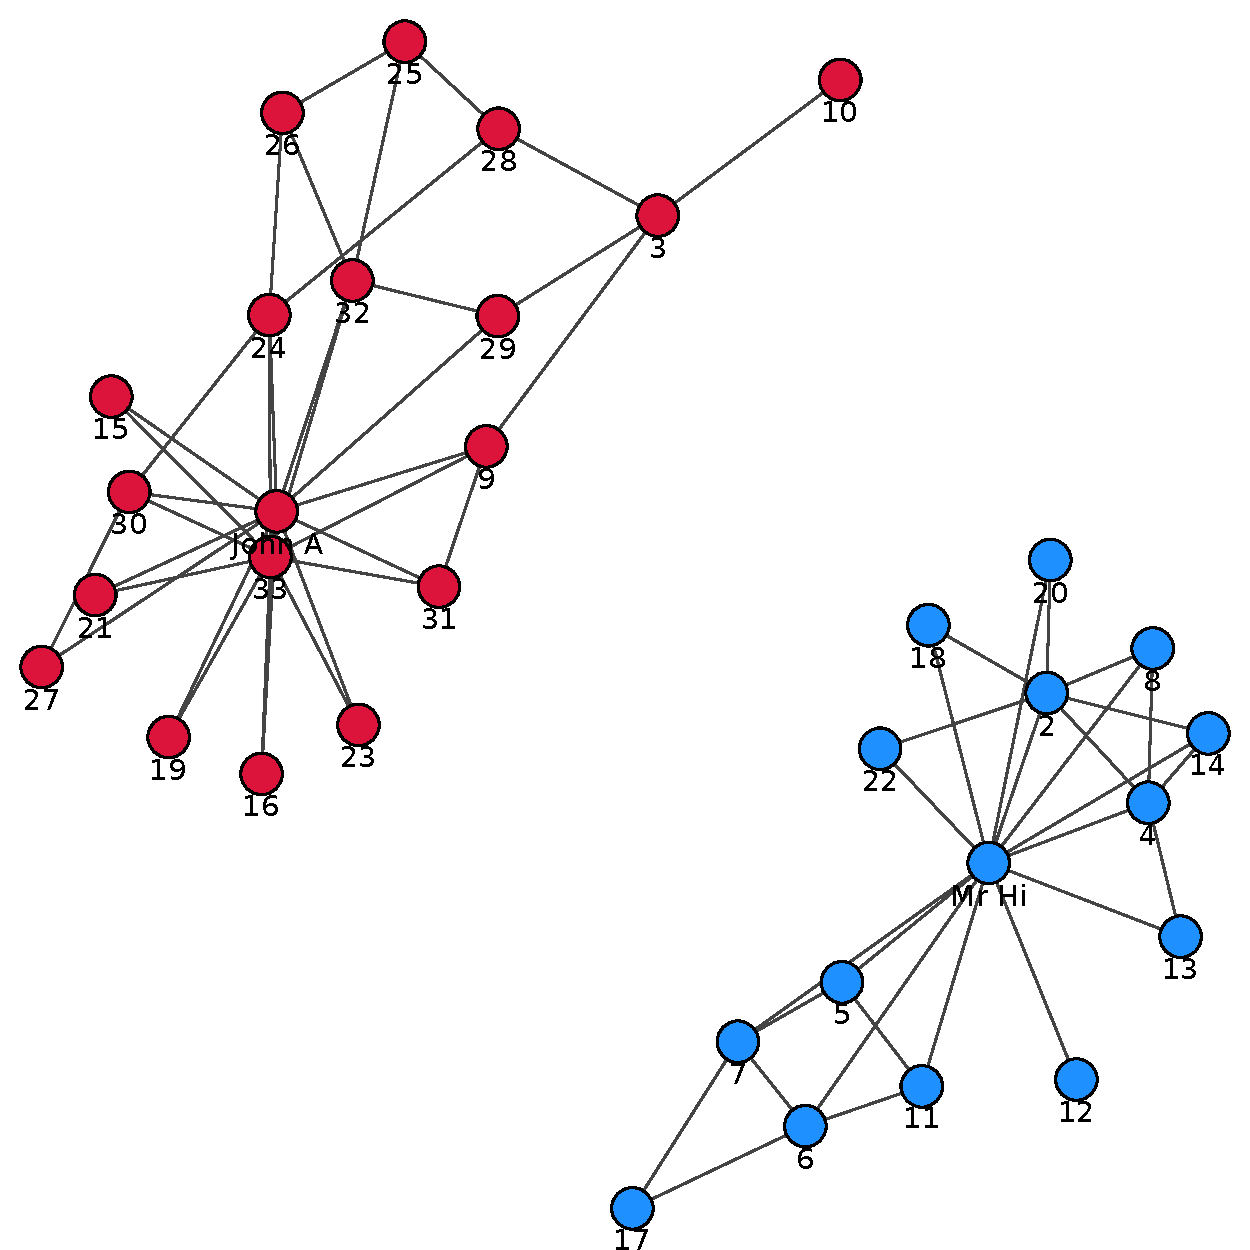
\includegraphics[scale=0.55, keepaspectratio=true]{figures/graphs/GraphWith2Groups.pdf}
\caption{Output of Girvan Newman algorithm which divides the Karate Club Graph divided into 2 groups}
\label{fig:q1fig12}
\end{center}
\end{figure}
\newpage
\item Comparison between the `Faction graph' and the resultant Karate Club split graph generated from `Girvan Newman' algorithm is illustrated in \ref{Table:q1table1}
\begin{table}

\label{Table:q1table1}
\begin{center}
\begin{tabular}{| c | c || c | c |}
\hline
Faction Graph & Girvan Newman Graph & Faction Graph & Girvan Newman Graph\\ \hline

Group 1 & & Group 2&  \\ \hline
John A &John A & Mr.Hi & Mr.Hi \\ \hline
- & 3 & 2 & 2 \\ \hline
9 & 9 & 3 & - \\ \hline
10 & 10 & 4 & 4 \\ \hline
15 & 15 & 5 & 5\\ \hline
16 & 16 & 6 & 6  \\ \hline
19 & 19 & 7 & 7  \\ \hline
21 & 21 & 8  & 8 \\ \hline
23 & 23 & 11 & 11\\ \hline
24 & 24 & 12 & 12\\ \hline
25 & 25 & 13 & 13\\ \hline
26 & 26 & 14 & 14\\ \hline
27 & 27 & 17 & 17\\ \hline
28 & 28 & 18 & 18\\ \hline
29 & 29 & 20 & 20\\ \hline
30 & 30 & 22& 22\\ \hline
31 & 31 & &\\ \hline
32 & 32 & &\\ \hline
33 & 33 & &\\ \hline

\end{tabular}
\end{center}
\end{table}
\item By looking at the table, We can say that all the nodes are same except from node 3. By this we can conclude that the mathematical model matches almost with the reality.
\newpage
\item This code is listed in Listing \ref{lst:q1code1}
\textbf{Code Listing}
\lstinputlisting[language=Python,caption=Python code which implements Girvan Newman algorithm to divide Karate Club Graph into groups of `2' `3' `4' and `5',frame=single,breaklines=true,label=lst:q1code1,captionpos=b,numbers=left,showspaces=false,showstringspaces=false,basicstyle=\footnotesize]{src/girvanNewman.py}
\end{itemize}



